    \begin{subfigure}[c]{0.4\textwidth}
    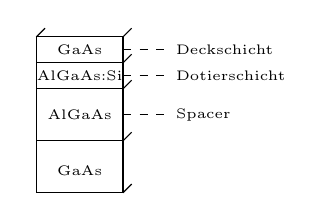
\begin{tikzpicture}[scale=1.1]
        % Heterostruktur Aufbau
        \draw (0,0) rectangle (1,1.8);
        % Striche
        \draw (0,0.6) -- (1,0.6);
        \draw (0,1.2) -- (1,1.2);
        \draw (0,1.5) -- (1,1.5);
        % 3D Striche
        \draw (0,1.8) -- (0.1,1.9);
        \draw (1,1.8) -- (1.1,1.9);
        \draw (1,1.5) -- (1.1,1.6);
        \draw (1,1.2) -- (1.1,1.3);
        \draw (1,0.6) -- (1.1,0.7);
        \draw (1,0) -- (1.1,0.1);
        % Beschriftung
        \draw (0.5,0.25) node {\tiny \ch{GaAs}};
        \draw (0.5,0.9) node {\tiny \ch{AlGaAs}};
        \draw (0.5,1.35) node {\tiny \ch{AlGaAs:Si}};
        \draw (0.5,1.65) node {\tiny \ch{GaAs}};
        % gestrichelte Linien
        \draw [dashed] (1,1.65) -- (1.5,1.65);
        \draw [dashed] (1,1.35) -- (1.5,1.35);
        \draw [dashed] (1,0.9) -- (1.5,0.9);
        % Beschriftung aussen
        \draw (1.5,1.65) node[anchor=west] {\tiny Deckschicht};
        \draw (1.5,1.35) node[anchor=west] {\tiny Dotierschicht};
        \draw (1.5,0.9) node[anchor=west] {\tiny Spacer};
    \end{tikzpicture}
    \end{subfigure}
    \begin{subfigure}[c]{0.4\textwidth}
        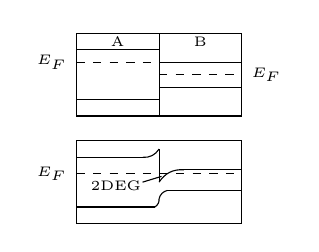
\begin{tikzpicture}[scale=1.05]
            % Halbleiter A
            \draw (1.5, 0) rectangle (2.5,1);
            \draw (1.5, 0.2) -- (2.5,0.2);
            \draw (1.5,0.8) -- (2.5,0.8);
            \draw [dashed] (1.5,0.65) -- (2.5,0.65);
            \draw (1.5,0.65) node[anchor=east] {\tiny $E_F$};
            \draw (2,0.9) node {\tiny A};
            % Halbleiter B
            \draw (2.5, 0) rectangle (3.5,1);
            \draw (2.5, 0.35) -- (3.5,0.35);
            \draw (2.5,0.65) -- (3.5,0.65);
            \draw [dashed] (2.5,0.5) -- (3.5,0.5);
            \draw (3.5,0.5) node[anchor=west] {\tiny $E_F$};
            \draw (3,0.9) node {\tiny B};
            % Heterostruktur
            \draw (1.5,-1.3) rectangle (3.5,-0.3);
            \draw [dashed] (1.5,-0.7) -- (3.5,-0.7);
                % Leitungsband
            \draw (1.5,-0.5) -- (2.3,-0.5);
            \draw (2.3,-0.5) to[bend right] (2.5,-0.4); 
            \draw (2.5,-0.4) -- (2.5,-0.8);
            \draw (2.5,-0.8) to[bend left] (2.8,-0.65);
            \draw (2.8,-0.65) -- (3.5,-0.65);
            \draw (2.5,-0.7) -- (2.6,-0.7);
                % Valenzband
            \draw (1.5,-1.1) -- (2.45,-1.1);
            \draw (2.45,-1.1) to[bend right] (2.5, -1.0);
            \draw (2.5,-1.0) to[bend left] (2.6,-0.9);
            \draw (2.6,-0.9) -- (3.5,-0.9);
                % Beschriftung
            \draw (2.3,-0.8) -- (2.53,-0.73);
            \draw (2.4,-0.85) node[anchor=east] {\tiny 2DEG};
            \draw (1.5,-0.7) node[anchor=east] {\tiny $E_F$};
        \end{tikzpicture}
    \end{subfigure}
